\documentclass[14pt, a4paper]{extreport}

\usepackage{susu}

% ====================================================================================================
\begin{document}

\author{Савонин~М.В.}
\group{211}
\task{2}
\maketitle

% ====================================================================================================
\chapter{Задание}

\begin{enumerate}

	\item
	Написать программу для создания множества точек и построения отрезка между двумя наиболее удаленными друг от друга точками множества. Для задания координат точек использовать генератор псевдослучайных чисел. Интерфейс программы должен содержать следующие элементы управления:
	\begin{itemize}
		\item создание множества точек;
		\item построение решеия;
		\item сохранение результата в файл;
		\item выход из программы.
	\end{itemize}

\end{enumerate}

% ====================================================================================================
\chapter{Математическая модель}

Пусть $x_0$, $y_0$, $w$, $h$ -- соответственно координаты левого верхнего угла, ширина и высота прямоугольной области.
При генерации точек мы выбираем координаты в диапозоне $x_0$+50 < x < $w$-50 и $y_0$+50 < y < $h$-50.
Так же координаты должны быть (x > 250 и y < 260) или (85 < x > 230 и y < 130) чтобы не попасть в лес или озеро на карте.
\par Перебирая все точки находим самые дальние вычисляя расстояние между ними по формуле $ \sqrt{\left(x_1-x_2\right)^2+\left(y_1-y_2\right)^2} $

% ====================================================================================================
\chapter{Текст программы}

\noindent Файл main.cpp
\lstinputlisting{source/main.cpp}
\pagebreak
\hrulefill

\noindent Файл task.h
\lstinputlisting{source/task.h}
\hrulefill

\noindent Файл task.cpp
\lstinputlisting{source/task.cpp}
\hrulefill

\noindent Файл control.h
\lstinputlisting{source/control.h}
\hrulefill

\noindent Файл control.cpp
\lstinputlisting{source/control.cpp}

% ====================================================================================================
\chapter{Результат работы}

\begin{figure}[h!]
	\centering
	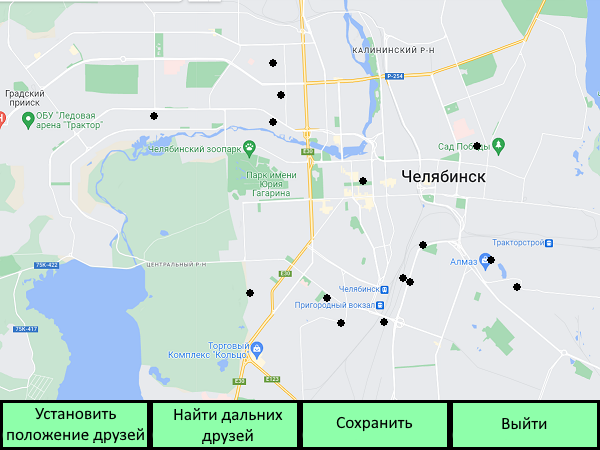
\includegraphics[width = 12cm]{image/image_1}
  \caption{Результат выполнения программы (функция creatPoint, кнопка "Установить положение друзей")}
\end{figure}

\begin{figure}[h!]
	\centering
	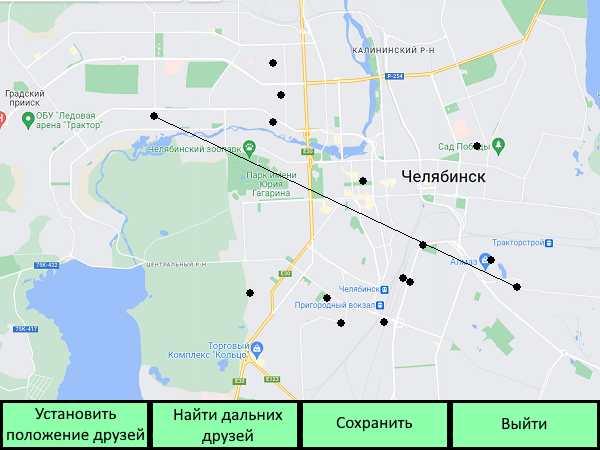
\includegraphics[width = 12cm]{image/image_2}
  \caption{Результат выполнения программы (функция treat, кнопка "Найти дальних друзей")}
\end{figure}

% ====================================================================================================
\end{document}